% \documentclass[11pt,a4paper,DIV=12]{scrartcl}
% \usepackage[utf8]{inputenc}
% \usepackage{fouriernc}
% \usepackage[T1]{fontenc}
% \usepackage[]{babel}
% \usepackage[hidelinks]{hyperref}
% \usepackage{natbib}
% \usepackage{url}
% \usepackage{amsmath}
% \usepackage{amsfonts}
% \usepackage{amssymb}
% \usepackage{trfsigns}
% \usepackage{nicefrac}
% \usepackage{graphicx}
% \usepackage{subcaption}
% \usepackage{xcolor}
% \usepackage{comment}
% \usepackage{mdframed}
% \usepackage{tikz,circuitikz,pgfplots}

% \usetikzlibrary{shapes.misc}
% \tikzset{cross/.style={cross out, draw,
%          minimum size=2*(#1-\pgflinewidth),
%          inner sep=0pt, outer sep=0pt}}

% \usetikzlibrary{matrix}

% \bibliographystyle{dinat}

% \numberwithin{equation}{section}
% \numberwithin{figure}{section}

% \newcommand\fsd{\mathrm{d}} %der/int operator
% \newcommand{\sysH}[1]{\mathcal{H}{\{#1\}}}  % system operator
% \renewcommand{\vec}[1]{\mathbf{#1}} %vector
% \newcommand{\eq}[1]{Eq. (\ref{#1})} %ref equation
% \newcommand{\fig}[1]{Fig. \ref{#1}} %ref figure
% \newcommand{\red}{\textcolor{red}}
% \newcommand{\blue}{\textcolor{blue}}

% %Sha symbol:
% \DeclareFontFamily{U}{wncy}{}
% \DeclareFontShape{U}{wncy}{m}{n}{<->wncyr10}{}
% \DeclareSymbolFont{mcy}{U}{wncy}{m}{n}
% \DeclareMathSymbol{\Sha}{\mathord}{mcy}{"58}

% %matplotlib colors:
% \definecolor{C0}{HTML}{1f77b4}
% \definecolor{C1}{HTML}{ff7f0e}
% \definecolor{C2}{HTML}{2ca02c}
% \definecolor{C3}{HTML}{d62728}
% \definecolor{C7}{HTML}{7f7f7f}

% \specialcomment{Ziel}{\begin{mdframed}[backgroundcolor=C2!10] \textit{Aim}\\\noindent}{\end{mdframed}\noindent}
% \specialcomment{Werkzeug}{\begin{mdframed}[backgroundcolor=C7!10] \textit{Tools}\\\noindent}{\end{mdframed}\noindent}
% \specialcomment{Ansatz}{\begin{mdframed}[backgroundcolor=C3!10] \textit{Ansatz}\\\noindent}{\end{mdframed}\noindent}
% \specialcomment{ExCalc}{\begin{mdframed}[backgroundcolor=C1!10]\noindent \textit{Calculus}\\\noindent}{\end{mdframed}\noindent}
% \specialcomment{Loesung}{\begin{mdframed}[backgroundcolor=C0!10] \textit{Solution}\\\noindent}{\end{mdframed}\noindent}

% %\excludecomment{Ziel}
% %\excludecomment{Werkzeug}
% %\excludecomment{ExCalc}

% %------------------------------------------------------------------------------
% \title{Signal- und Systemtheorie\\
% Übung\thanks{
% This tutorial is provided as Open Educational Resource (OER), to be found at
% \url{https://github.com/spatialaudio/signals-and-systems-exercises}
% accompanying the OER lecture
% \url{https://github.com/spatialaudio/signals-and-systems-lecture}.
% %
% Both are licensed under a) the Creative Commons Attribution 4.0 International
% License for text and graphics and b) the MIT License for source code.
% %
% Please attribute material from the tutorial as \textit{Frank Schultz,
% Continuous- and Discrete-Time Signals and Systems - A Tutorial Featuring
% Computational Examples, University of Rostock} with
% \texttt{main file, github URL, commit number and/or version tag, year}.
% }
% \\
% \small Universität Rostock Vst.-Nr. 24015}
% %
% \author{Dr. Frank Schultz, Prof. Sascha Spors\\
% \small Institut für Nachrichtentechnik (INT)\\
% \small Fakultät für Informatik und Elektrotechnik (IEF)\\
% \small Universität Rostock
% }
% %
% \date{Sommersemester 2020, Version: \today}
% %------------------------------------------------------------------------------
% \begin{document}
% \maketitle
% \tableofcontents
% \setcounter{section}{4}
% %##############################################################################
% %##############################################################################

\newpage
\section{LTI Systems in Spectral Domain: The Level Response}
\noindent In this exercise we will add a very important view onto the things
going on in SigSys: we will learn how to interpret LTI systems in the spectral
domain, also called the frequency domain. By that we start to get the bigger
picture of SigSys and we will be able to sort things that we've already mastered
in basic electrical engineering courses.

Thus, in this exercise we will learn how to draw a Bode plot of the
magnitude (more precisely the level in Decibel) over frequency.
Although our computers would (in later practice indeed will)
perform this task for us, it is good to know what's going on in detail.
Most likely we are already familiar with the Bode plot from analysis of RLC
circuits in electrical engineering. We will see how this earlier viewpoint will
perfectly fit into the SigSys world. We should start thinking of LTI systems as
poles and zeros in the Laplace domain and what they are doing in terms
of the frequency response, the impulse and step response and of course to
any other arbitrary input signal.

\begin{mdframed}
SigSys for an LTI system denoted with operator $\mathcal{H}$ is in essence described
by the three most important equations / relationships
\begin{align}
&h(t) = \mathcal{H}\{\delta(t)\}\\
&h(t) \,\laplace\, H(s)\\
&y(t) = x(t) \ast h(t) \,\laplace\, Y(s) = X(s) \cdot H(s),
\end{align}
which we already know very good.
%
It includes the concept of the impulse response, its convolution with input
signal $x$ to yield the output signal $y$, and the equivalence in the Laplace
domain using multiplication with the transfer function $H$.
If we are interested in the steady state of the system (in practice we are quite often),
we can evaluate the Fourier transform as special case of Laplace transform
\begin{align}
&h(t) = \mathcal{H}\{\delta(t)\}\\
&h(t) \,\laplace\, H(s)\big|_{s=\im\omega}\\
&y(t) = x(t) \ast h(t) \,\laplace\, Y(s)\big|_{s=\im\omega} = X(s)\big|_{s=\im\omega} \cdot H(s)\big|_{s=\im\omega}.
\end{align}
%
We should note that the Fourier domain by itself also holds in general
\begin{align}
&h(t) = \mathcal{H}\{\delta(t)\}\\
&h(t) \,\fourier\, H(\im\omega)\\
&y(t) = x(t) \ast h(t) \,\fourier\, Y(\im\omega) = X(\im\omega) \cdot H(\im\omega).
\end{align}
\end{mdframed}

\clearpage

\begin{figure}
\centering
\begin{tikzpicture}
\def \axisLength {4}
\def \tic {0.05}
\def \sigmaz {3/4}
\def \omegaz {1}
\def \convAbsz {-\sigmaz}
\fill[C2!50] (\convAbsz,-\axisLength/2)--(\convAbsz,\axisLength/2)
decorate [decoration={snake,segment length=15pt,amplitude=1pt}]
{(\convAbsz,\axisLength/2)--
(\axisLength/2,\axisLength/2)--
(\axisLength/2,-\axisLength/2)--
(\convAbsz,-\axisLength/2)};
\draw[->] (-\axisLength/2,0)--(\axisLength/2,0) node[right]{\small$\Re\{s\}$};
\draw[->] (0,-\axisLength/2)--(0,\axisLength/2) node[above]{\small$\Im\{s\}$};
\draw[-, C3] (0,+\axisLength/2+1/2)--(0,-\axisLength/2-1/2) node[below]{\small$\textcolor{C3}{H(\im\omega)}$};
\draw[C0, ultra thick] (-\sigmaz,+\omegaz) node{\Huge $\times$};
\draw[C0, ultra thick] (-\sigmaz,-\omegaz) node{\Huge $\times$};
\draw (-\sigmaz,\tic)--(-\sigmaz,-\tic) node[below]{$-\frac{3}{4}$};
\draw (-\tic,\omegaz) -- (\tic,\omegaz) node[right]{$+1$};
\draw (-\tic,-\omegaz) -- (\tic,-\omegaz) node[right]{$-1$};
\draw (1.25,+2.25) node[C2!75]{ROC};
\draw (1.25,1.75) node[]{$H_0=\frac{25}{16}$};
\end{tikzpicture}
\caption{Pole-zero map with region of convergence (ROC) for the causal LTI system
$H(s) = \left[\frac{16}{25} s^2 + \frac{24}{25} s + 1\right]^{-1}$.
The $\Im\{s\}$-axis is included in the ROC, thus $H(\im\omega)$ can be evaluated as
frequency response of the LTI system.}
\label{fig:pzmap_44EB4169E9}
\end{figure}



From exercise 3 we know a special 2nd order lowpass LTI system very well.
Due to our detailed analytical treatment, we can qualify and quantify this system
with the following SigSys tools:
\begin{itemize}
  \item ODE: $\frac{16}{25} \ddot{y}(t) + \frac{24}{25} \dot{y}(t) + y(t) = x(t)$
  \item Impulse response: $h(t) = \frac{25}{16} \mathrm{e}^{-\frac{3}{4} t} \sin(t) \epsilon(t)$
  \item Step response: $h_\epsilon(t)=\left[1
  - \e^{-\frac{3}{4} t} \cos(t)
  - \frac{3}{4}\e^{-\frac{3}{4} t} \sin(t) \right]\epsilon(t)$
  \item Transfer function:
  $H(s) = \frac{1}{\frac{16}{25} s^2 + \frac{24}{25} s + 1}\Laplace h(t)
  \qquad\text{ROC: }\Re\{s\}>-\frac{3}{4}$
  \item Pole-zero map in \fig{fig:pzmap_44EB4169E9} and in 3D
  \fig{fig:bodeplot_example_approximations_pzmaps3D_44EB4169E9}
  \item Frequency response $H(s)\big|_{s=\im\omega}$:
  $H(\im\omega) = \frac{1}{-\frac{16}{25}\omega^2 + \frac{24}{25}\im\omega  + 1}
  \Fourier h(t)$
  \item Magnitude response over angular frequency: $|H(\im\omega)|$
  \item Phase response over angular frequency: $\angle H(\im\omega)$ in radian or degree
  \item Level over angular frequency: $20 \log_{10}|H(\im\omega)|$ in Dezibel
\end{itemize}

We will have a detailed look at the last item in this exercise.
%In the next exercise 6, we will
%discuss the phase response a bit more.

Based on this long list, we will get a feeling that although the fundamentals
lie in the ODE representation (remember that we started there in exercise 1),
the ODE entry is comparably lost in comparison to all the other SigSys tools,
that should simplify our engineering lives.

\begin{mdframed}
In essence, when discussing an LTI system in time and frequency domain, the
graphs of \fig{fig:pzmap_44EB4169E9} and \fig{fig:lowpass2nd_44EB4169E9}
will help to interpret the system characteristic from different viewpoints.
Pole/zero/gain map, impulse, step, level and phase response are the most important
ones and actually must haves.
The so called Nyquist plot and the so called Nichols plot are common in
control system engineering.
We need to learn what to see in these graphs.
\end{mdframed}




\begin{figure}
  \includegraphics[width=\textwidth]{../laplace_system_analysis/lowpass2nd_44EB4169E9.pdf}
  \caption{Full SigSys picture of the 2nd order lowpass system from
  \fig{fig:pzmap_44EB4169E9}. \texttt{lowpass2nd\_44EB4169E9.ipynb}}
  \label{fig:lowpass2nd_44EB4169E9}
\end{figure}


\begin{figure}
  \includegraphics[width=\textwidth]{../laplace_system_analysis/bodeplot_example_approximations_pzmaps3D_44EB4169E9.pdf}
  \caption{3D view of Laplace domain for 2nd order lowpass system from
  \fig{fig:pzmap_44EB4169E9}.
  The green line corresponds to the magnitude response along $-\omega...+\omega$.
  Typically we are only interested in the physical frequencies $\omega\geq0$ and
  very often the frequency axis is logarithmic additionally.
  \texttt{bodeplot\_example\_approximations\_pzmaps3D.ipynb}}
  \label{fig:bodeplot_example_approximations_pzmaps3D_44EB4169E9}
\end{figure}




\begin{figure}
  \includegraphics[width=\textwidth]{../laplace_system_analysis/bodeplot_examples_pt1_element.pdf}
  \caption{Full SigSys picture of the \textbf{1st order lowpass system from
  exercise 3.4} with $T_\mathrm{RC} = \frac{1}{\omega_\mathrm{RC}} = 1$ s.
  \texttt{bodeplot\_examples.ipynb}}
  \label{fig:bodeplot_examples_pt1_element}
\end{figure}



\newpage
\subsection{Lowpass 2nd Order / PT2 Element}
\label{sec:44EB4169E9}
\begin{Ziel}
We should explore the Bode plot approximations based on zeros and poles.
In pre-computer decades this was a vivid job of signal
processing and control system engineering.
Although nowadays a computer calculates the frequency response faster and plots it
probably nicer, we should be able to grasp the picture of the frequency response
by rough calculation. Furthermore, by doing this we learn how zeros and poles
of an LTI system actually  contribute to the frequency response. This knowledge
is indeed basic engineering stuff, and that's why we do it here in detail.
\end{Ziel}
\textbf{Task} {\tiny 44EB4169E9}:
Let us consider the Laplace transform (note that we already known this from
exercise 3)
\begin{align}
\label{eq:H_ODE}
H(s) = \frac{1}{\frac{16}{25} s^2 + \frac{24}{25} s + 1}\qquad\text{ROC: }
\Re\{s\}>-\frac{3}{4}
\end{align}
as transfer function of a causal LTI system.
%
We shall discuss the level response in terms of the (approximated) Bode plot.
%
Note: The frequency response exists only if the $\Im(s)$-axis is included
in the region of convergence (ROC), which is the case here.

\begin{Werkzeug}
A potential and nice approach to solve the task is given in the Appendix.
\end{Werkzeug}
\begin{Ansatz}
Quasi-standardized notation with coefficients $b\in\mathbb{R}$ for the numerator and
$a\in\mathbb{R}$ for the denominator
\begin{align}
H(s) = \frac{b_2 s^2+b_1 s + b_0}{a_2 s^2+a_1 s +a_0}
\end{align}
Thus, for
$H(s) = \frac{1}{\frac{16}{25} s^2 + \frac{24}{25} s + 1}$,
the coefficients are given as
$b_0 = 1$, $a_0=1$, $a_1 = \frac{24}{25}$ and
$a_2 = \frac{16}{25}$, $b_1=b_2=0$.
%
In pole/zero notation this could be reformulated
\begin{align}
H(s) =& H_0 \frac{1}{(s-s_{\infty,1}) (s-s_{\infty,2})}\\
H(s) =& \frac{25}{16}\cdot\frac{1}{[s-(-\frac{3}{4}+\im)] [s-(-\frac{3}{4}-\im)]}
=
\frac{25}{16}\cdot\frac{1}{s^2 + \frac{24}{16} s  + \frac{25}{16}}
\end{align}
when considering $b_{m=0} = 1$ and $a_{n=2}=\frac{16}{25}$ for
$H_0 = \frac{b_{M=0}}{a_{N=2}}=\frac{25}{16}$ and the pole pair
$s_{\infty,1,2} = -\frac{3}{4} \pm \im$.
\end{Ansatz}

\begin{mdframed}
\textit{Some notes on generalization}


Our system under discussion exhibits a complex conjugate pole pair and no zeros,
and thus can be given as
\begin{align}
H(s) =
\frac{K}{\frac{1}{\omega_0^2} s^2 + \frac{2 D}{\omega_0} s + 1}=
\frac{K \omega_0^2}{s^2 + 2 D \omega_0 s + \omega_0^2} =
\frac{H_0}{s^2 + \frac{\omega_0}{Q_{\infty,1}} s + \omega_0^2} =
\frac{H_0}{s^2 + \frac{|s_{\infty,1}|}{Q_{\infty,1}} s + |s_{\infty,1}|^2}.
\end{align}
and
\begin{align}
\label{eq:Hs_general}
H(s) = \frac{K}{\frac{1}{\omega_0^2} s^2 + \frac{2 D}{\omega_0} s + 1}
= \frac{K}{\tau_0^2 s^2 + 2 D \tau_0 s + 1}.
\end{align}
These are common general notations of this 2nd order system.

The so called damping factor $0\leq D \leq 1$ realizes differently damped,
stable LTI systems for a chosen cutoff frequency $\omega_0=\nicefrac{1}{\tau_0}$.
Furthermore, we can link the so called pole quality $Q_{\infty,1} $ to the damping factor
$D$ by
\begin{align}
Q_{\infty,1} = \frac{1}{2 D}.
\end{align}
Both qualities allow for convenient interpretation and discussion of the
system characteristics. Note the special case of equal quantity
$D = Q_{\infty,1} = \frac{1}{\sqrt{2}}$, which yields a 2nd order
lowpass filter with so called Butterworth characteristics.
%\begin{figure}[b!]
%\centering
\begin{center}
\begin{tikzpicture}
\draw [-latex] (-2,0) -- (3.5,0) node [right]  {$\Re(s)$};
\draw [-latex] (0,-2) -- (0,2) node [above] {$\Im(s)$};
\draw[dashed] (0,0) -- node[pos=0.7, right] {$\omega_0$}(135:2) node[solid, fill=white, cross=6pt, draw=blue, ultra thick] {};
\draw[dashed] (0,0) -- node[pos=0.6, above right] {$ $}(-135:2) node[solid, fill=white, cross=6pt, draw=blue, ultra thick] {};
\draw[dashed] (-1.4142,0) -- (-1.4142,+1.4142);
\draw[dashed] (-1.4142,-1.4142) -- (-1.4142,-0.5) node [left, above] {$-\sigma_0$};
\draw[dashed] (-1.4142,+1.4142) -- (0,+1.4142) node [right] {$+\omega_D$};
\draw[dashed] (-1.4142,-1.4142) -- (0,-1.4142) node [right] {$-\omega_D$};
\draw[black, -latex] (-0.75,0.75) arc (135:180:1);
\node at (1.9,1) {$\omega_D = \omega_0 \sqrt{1-D^2}$};
\node at (1.3,0.5) {$\sigma_0 = D \omega_0$};
\node at (-0.7,0.25) {$\alpha$};
\node at (1.4,-0.25) {$\cos \alpha = D$};
\end{tikzpicture}
%\caption{Pole-zero map of 2nd order LTI system under discussion with a complex
%conjugate pole pair.}
%\label{fig:sketch_lambda_plane}
%\end{figure}
%
\end{center}
%
For $D=0$ the poles are located on $\Im(s)$-axis (i.e. semi-stable),
the system behaves very resonant at $\omega_0$.
For higher $D$ this resonant characteristics becomes increasingly
damped, since the poles increasingly move away from the $\Im(s)$-axis.
%
This is why $D$ is typically termed damping factor. It is directly
proportional to $\sigma_0$ of the system's poles shown in the figure above.
We can write this as $D\propto \sigma_0$.

Note, that in \eq{eq:Hs_general} the first version using $\omega_0$ is
common in filter design, whereas the second version with the time
constant $\tau_0$ is often used in controlling engineering.
%
This is meaningful since in filter design often the frequency response is to be
optimised, whereas a controller is rather optimised for a dedicated
temporal behaviour.
%
The system under discussion is thus called either a lowpass of 2nd order
(frequency design view) or a PT$_2$-element (control system view).
This is just naming dealing with the same LTI system.
Despite of that, we need to figure out how to describe its behaviour in the
frequency domain in the following.
A valuable reference for further reading on the topic are Chapter 6.5.2
in Oppenheim, Willsky, Nawab (1997): "\textit{Signals \& Systems}", Prentice Hall,
Upper Saddle River NJ (USA), 2nd edition
or Fliege, N. (1991): "\textit{Systemtheorie}", Teubner, Stuttgart.
%
%
%

From the pole-zero map in the $s$-domain given above
%\ref{fig:sketch_lambda_plane}
we can deduce helpful variables
\begin{equation}
D = \cos \alpha = \frac{\sigma_0}{\omega_0},\qquad
\omega_D^2 = \omega_0^2 (1-D^2) \quad \rightarrow \quad \omega_D = \omega_0
\sqrt{1-D^2}.
\end{equation}
where we assume $\sigma_0\geq 0$, $\omega_D\geq 0$, $\omega_0\geq 0$.
%
The two poles of the LTI system under discussion then can be given in terms of
these variables
\begin{align}
s_{\infty,1,2} = -\sigma_0 \pm \im\,\omega_D
\end{align}
%
Thus, from the given quantities we find for our special example
\begin{equation}
K=1, \qquad \omega_0^2 = \frac{25}{16} \cdot \frac{1}{\text{s}^2}
\rightarrow \omega_0 = \frac{5}{4} \cdot \frac{\text{1}}{\text{s}},
\qquad D = \frac{3}{5},\qquad
Q_{\infty,1} = \frac{5}{6}
\end{equation}
and by that the real and imaginary parts of the poles
\begin{equation}
\sigma_0 = \frac{3}{4}\cdot \frac{\text{1}}{\text{s}},\qquad
\omega_D = 1 \cdot \frac{\text{1}}{\text{s}},
\end{equation}
%
and thus $s_{\infty,1,2} = -\frac{3}{4} \pm \im$
omitting the physical unit \textit{second} in the following.
%
Note that the distance $|s_{\infty,1,2}| = \omega_0=\frac{5}{4}$, which is later required.
%
The ROC is $\Re\{s\}>-\frac{3}{4}$ and thus includes the $\Im(s)$-axis.
%
We therefore can evaluate the frequency response of the system, which is the
Fourier transform of the impulse response,
which is a special case of $H(s)$ using $s=\sigma+\im\omega$ for $\sigma=0$.
\end{mdframed}







\begin{ExCalc}
The poles constitute a complex conjugate pair, thus
$|s_{\infty,1}| = |s_{\infty,2}| = \frac{5}{4}$, $|s_{\infty,1}|^2 = |s_{\infty,2}|^2 = \frac{25}{16}$.
%
With \eq{eq:H0tilde}
\begin{align}
\tilde{H_0} = \frac{H_0}{|s_{\infty,1}|^2} = \frac{\nicefrac{25}{16}}{\nicefrac{25}{16}} = 1
\end{align}
and the suitable prototypes \eq{eq:Hs_sorted_for_Bode_dB_gain} and \eq{eq:Hs_sorted_for_Bode_dB_ccpole}
we get
\begin{align}
20 \text{lg} |H(s)| =
+20 \text{lg} |\tilde{H_0}|
-20 \text{lg} \bigg|\frac{s^2}{|s_{\infty,1}|^2} + \frac{s}{|s_{\infty,1}| Q_{\infty,1}} + 1\bigg|.
\end{align}
Since here we have $20 \text{lg} |\tilde{H_0}|=0\mathrm{dB}$ we only need
\begin{align}
20 \text{lg} |H(s)| =
-20 \text{lg} \bigg|\frac{s^2}{|s_{\infty,1}|^2} + \frac{s}{|s_{\infty,1}| Q_{\infty,1}} + 1\bigg|.
\end{align}
This directly corresponds to the prototype \eq{eq:Hs_sorted_for_Bode_dB_ccpole}, which
is schematically depicted in Fig. \ref{fig_bode_mag_conj_poles}.
For
\begin{align}
\frac{s^2}{|s_{\infty,1}|^2} + \frac{s}{|s_{\infty,1}| Q_{\infty,1}} + 1
\end{align}
we already know that $Q_{\infty,1}=\frac{5}{6}$, which however is irrelevant for the
approximated Bode plot.
%
%However we are aware that this conjugate complex pole pair corresponds
%to the case of underdamping.
%
We are ready to design the approximated Bode plot for the magnitude.

In essence, we recast the Laplace transform $H(s)$ to prototypes of transfer function
from which we know the (simple) frequency responses. In the dB-domain
we then just add them up to yield the final frequency response in dB.
This corresponds to a series connection, also known as filter cascade
$H(s)=H_1(s)\cdot H_2(s)\cdot\dots$, of the used prototypes.

%
\end{ExCalc}
\begin{Loesung}
The Bode plot of \eq{eq:H_ODE} is depicted in
\fig{fig:bodeplot_example_approximations_44EB4169E9}.


%
In \fig{bodeplot_example_approximations_level_44EB4169E9} the approximation is plotted as
black graph with a slope of -40 dB per decade starting at
$\omega_0 = |s_{\infty,1}|=\frac{5}{4}$.
The slope is also often referenced to frequency doubling, i.e. here
-12 dB/octave\footnote{Slopes correspond to the order $o$ of a lowpass system,
hence $-o\cdot 20$ dB/decade, $-o\cdot 6$ dB/octave.
We deal with $o=2$ order system due to two poles.},
cf. this at frequencies $\omega=2.5, 5, 10$ rad/s in the plot.

The exact solution with $Q_{\infty,1}=\frac{5}{6}$ and thus exact magnitude plot
is depicted as olive graph. This pole quality leads to $\approx 0$ dB at
$\omega_D=1$ rad/s and a very flat response for frequencies up to $\omega_D$
with only very slight overshoot at around $\omega = 0.5$ to $0.8$ rad/s.
Note that by decreasing $Q\rightarrow 0.5$ (thus $D\rightarrow 1$)
the system becomes less resonant.
A special case---called Butterworth filter characteristic---is
$Q = \frac{1}{\sqrt{2}}$, where -3.01 dB at $\omega_0 = \frac{5}{4}$ rad/s is
obtained, cf. Fig. \ref{fig_bode_mag_conj_poles}.
By increasing $Q$ (thus $D\rightarrow 0$) a more resonant system characteristic at $\omega_0$ is achieved.
%
The phase response of the 2nd order lowpass under discussion is depicted
in \fig{bodeplot_example_approximations_phase_44EB4169E9}.
It exhibits typical phase shift of zero at very low frequencies near 0 rad/s and -180 deg phase at very high frequencies.
A phase shift of -90 deg is generally obtained at $\omega_0$ independently of
the pole quality.
This is the reason why $w_0$ is often referred to as the cut frequency
of the lowpass filter, since it marks the borderline between the two general
characteristics: $\omega \ll \omega_0$ defines the so called passband,
$\omega \gg \omega_0$ defines the so called stop band of the lowpass.
The transition
(the steepness of the slope and its style) between the two bands is
determined by the filter order (number of poles) and characteristics (position of poles within $s$-plane).
For details there are numerous book on filter design. The standard reference Tietze, U.; Schenk, Ch.; Gamm, E. (2008): "\textit{Electronic Circuits --- Handbook for Design and Applications}", Springer, 2nd ed. is a good starting point for filter design.

We are ready to play with poles in the Laplace domain.

The
input \verb|bode plot (1)/(16/25*s^2+24/25*s+1)|
to
\url{https://www.wolframalpha.com/}
is a convenient tool. Furthermore, the Jupyter notebooks
at

\url{https://github.com/spatialaudio/signals-and-systems-exercises/tree/master/laplace_system_analysis}

might be helpful.
\end{Loesung}

\begin{figure}[h!]
\centering
\subfloat[Level over frequency, cf. Fig. \ref{fig_bode_mag_conj_poles}.
Undamped natural frequency $\omega_0=\frac{5}{4}$ rad/s. $\omega_D=1$ rad/s,
$Q_\infty=\frac{5}{6}$, $D=\frac{3}{5}$.
This is a lowpass with slope of -40 dB/decade, i.e. -12 dB/octave
(cf. the markers $\omega=\frac{5}{2}$ rad/s and $\omega=5$ rad/s).
\label{bodeplot_example_approximations_level_44EB4169E9}]{%
\includegraphics[width=0.6\textwidth]{../laplace_system_analysis/bodeplot_example_approximations_level_44EB4169E9}
}

\subfloat[Phase over frequency.
Note -90 deg at $\omega_0$, 0 deg for $\omega \rightarrow 0 $ and -180 deg for
$\omega\rightarrow \infty$. \label{bodeplot_example_approximations_phase_44EB4169E9}]{%
\includegraphics[width=0.6\textwidth]{../laplace_system_analysis/bodeplot_example_approximations_phase_44EB4169E9}
}
\caption{Bode plot of LTI system \eq{eq:H_ODE}.
\texttt{bodeplot\_example\_approximations.ipynb}.}
\label{fig:bodeplot_example_approximations_44EB4169E9}
\end{figure}





\clearpage
\subsection{Bandpass 2nd Order}
\label{sec:590A7AFD51}
\begin{Ziel}
Another Bode diagram. Here we deal with a zero at the origin and two real
poles. The overall gain $\tilde{H}_0$ deviates from 1.
\end{Ziel}
\textbf{Task} {\tiny 590A7AFD51}: Discuss the frequency response in terms
of the (approximated) Bode plot for the causal LTI system
\begin{align}
H(s) = \frac{100 s}{10 s^2 + 101 s + 10}\qquad\text{ROC: }
\Re\{s\}>-\frac{1}{10}.
\end{align}
\begin{Werkzeug}
See Appendix.
\end{Werkzeug}
\begin{Ansatz}
We need to recast to pole/zero/gain representation
\begin{align}
H(s) = H_0\frac{s-s_{0,1}}{(s-s_{\infty,1})(s-s_{\infty,2})}
\end{align}
to handle a superposition of the frequency response prototypes shown in
\fig{fig:magbodeprototype}.
\end{Ansatz}

\begin{ExCalc}
For system interpretation we always need the poles, the zeros and the gain:

$s_0=0$,
$s_{\infty,1}=-\frac{1}{10}$,
$s_{\infty,2}=-10$

$|s_{\infty,1}|=\frac{1}{10}$,
$|s_{\infty,2}|=10$

$H_0=10$

\begin{center}
\begin{tikzpicture}
\centering
\def \axisLength {4}
\def \tic {0.05}
\def \sigmaz {1/2}
\def \omegaz {1}
\def \convAbsz {-\sigmaz}
\fill[C2!50] (\convAbsz,-\axisLength/2)--(\convAbsz,\axisLength/2)
decorate [decoration={snake,segment length=15pt,amplitude=1pt}]
{(\convAbsz,\axisLength/2)--
(\axisLength/2,\axisLength/2)--
(\axisLength/2,-\axisLength/2)--
(\convAbsz,-\axisLength/2)};
\draw[->] (-\axisLength/2-5,0)--(\axisLength/2,0) node[right]{\small$\Re\{s\}$};
\draw[->] (0,-\axisLength/2)--(0,\axisLength/2) node[above]{\small$\Im\{s\}$};
\draw[-, C3] (0,+\axisLength/2+1/2)--(0,-\axisLength/2-1/2) node[below]{\small$\textcolor{C3}{H(\im\omega)}$};
\draw[C0, ultra thick] (-5,0) node{\Huge $\times$};
\draw[C0, ultra thick] (-\sigmaz,0) node{\Huge $\times$};
\draw[C0, ultra thick] (0,0) node{\Huge $\circ$};
\draw (-\sigmaz,\tic)--(-\sigmaz,-\tic) node[below]{$-\frac{1}{10}$};
\draw (-5,\tic)--(-5,-\tic) node[below]{$-10$};
\draw (1.25,+2.25) node[C2!75]{ROC};
\draw (1.25,1.75) node[]{$H_0=10$};
\draw (-5,-1) node[]{not to scale};
\end{tikzpicture}
\end{center}

Checking:
\begin{align}
H(s) = H_0\frac{s-s_{0,1}}{(s-s_{\infty,1})(s-s_{\infty,2})} = 10\frac{(s-0)}{(s-(-0.1))(s-(-10))}
=\frac{100 s}{10 s^2 + 101 s + 10}.
\end{align}
%
Now we ware ready to elaborate the magnitude frequency response prototypes for this
LTI system in order to obtain the Bode plot approximation.
%
Four contributions from \eq{eq:Hs_sorted_for_Bode_dB_gain} to \eq{eq:Hs_sorted_for_Bode_dB_ccpole} need to be considered
\begin{align}
20\mathrm{lg}|H(s)| = 20\mathrm{lg}|\tilde{H_0}| + 20\mathrm{lg}|s| - 20\mathrm{lg}|\frac{s}{|s_{\infty,1}|}-1|
- 20\mathrm{lg}|\frac{s}{|s_{\infty,2}|}-1|,
\end{align}
and \eq{eq:H0tilde} becomes
\begin{align}
\tilde{H_0} = \frac{H_0}{|s_{\infty,1}| \cdot |s_{\infty,2}|} = 10 \rightarrow 20\mathrm{lg}|\tilde{H_0}| = 20 \mathrm{dB}.
\end{align}
Note: zeros or poles in the origin are not considered for calculation of $\tilde{H}_0$.
\end{ExCalc}
\begin{Loesung}

We draw the prototypes as level in dB over angular frequency $\omega$
\begin{itemize}
\item blue: 20 dB line frequency independent due to \eq{eq:Hs_sorted_for_Bode_dB_gain}
\item orange: 20dB/decade (12dB/octave) rising line due to the zero in the origin,
\eq{eq:Hs_sorted_for_Bode_dB_origin}
\item green: first real pole, thus -20dB/decade (-12dB/octave) starting from $|s_{\infty,1}| = \frac{1}{10}$, due to
\eq{eq:Hs_sorted_for_Bode_dB_pole}
\item red: second real pole, thus -20dB/decade (-12dB/octave) starting from $|s_{\infty,2}| = 10$, due to
\eq{eq:Hs_sorted_for_Bode_dB_pole}
\end{itemize}
We add up all these curves in the diagram. Due to log law this corresponds to the final approximation
in dB, shown in black, this is the approximated magnitude Bode plot.
The exact result is plotted in olive, this is the magnitude Bode plot.
The graphs are depicted in \fig{fig:bodeplot_example_approximations_590A7AFD51}.
The system has bandpass characteristics, which means very low and very high
frequencies are attenuated. Angular frequencies between 0.1 and 10 rad/s can pass
thru.
\end{Loesung}

\begin{figure}[h!]
\centering
\includegraphics[width=0.75\textwidth]{../laplace_system_analysis/bodeplot_example_approximations_590A7AFD51.pdf}
\caption{Level over frequency of 2nd order bandpass.
\texttt{bodeplot\_example\_approximations.ipynb}.}
\label{fig:bodeplot_example_approximations_590A7AFD51}
\end{figure}
















\clearpage
\subsection{Highpass 2nd Order with Resonance}
\label{sec:1EC316D8B2}
\begin{Ziel}
Just another Bode diagram to practice. Here we deal with two real zeros,
one of them is in the origin. Furthermore a conjugate complex pole pair has to be
considered. This results in the most curvy frequency response we have seen so far.
We get an idea on the placement of zeros and poles in the $s$-domain.
\end{Ziel}
\textbf{Task} {\tiny 1EC316D8B2}:  Discuss the frequency response in terms
of the (approximated) Bode plot for the causal LTI system
\begin{align}
H(s) = \frac{s^2+10 s}{s^2+\sqrt{2} s +1}\qquad\text{ROC: }
\Re\{s\}>-\frac{1}{\sqrt{2}}
\end{align}
\begin{Werkzeug}
The same as before. We should see the beauty of SigSys: we defined a system
in the Laplace domain completely detached from a RLC circuit or a ODE.
Although, it is good to know on which roots SigSys is founded, we don't need
any RLC circuit analogies to grasp the working principles, once we got into the
SigSys mindset. Congratulations, we've mastered a very important step in knowledge!
\end{Werkzeug}
\begin{Ansatz}
In practice most often causal systems are considered and the ROC is typically
not explicitly stated then, but assumes the ROC right of the most right pole(s).
If then \textbf{all poles are in the left} $s$-plane, the system is \textbf{stable},
which is the case here.
In other words: an unstable system does not include the $\Im\{s\}$-axis and therefore
no Fourier transform, and therefore no frequency responses exists, since unstable
is by definition not a steady state.

A 2nd order system is commonly denoted as
\begin{align}
H(s) = \frac{b_2 s^2+b_1 s + b_0}{a_2 s^2+a_1 s +a_0}
\end{align}
here with numerator coefficients $b_2 = 1, b_1 = 10, b_0=0$ and denominator
coefficients
$a_2 = 1, a_1 = \sqrt{2}, a_0=1$ with ROC: $\Re\{s\}>-\frac{1}{\sqrt{2}}$.
We can recast this in pole / zero representation
\begin{align}
H(s) = H_0\frac{(s-s_{0,1}) (s-s_{0,2})}{(s-s_{\infty,1})(s-s_{\infty,2})}
\end{align}
which is needed to draw the Bode approximation of the level over frequency.
\end{Ansatz}
\begin{ExCalc}
\begin{align}
&s_{0,1} = 0\rightarrow |s_{0,1}| = 0\\
&s_{0,2} = -10 \rightarrow |s_{0,2}| = 10\\
&s_{\infty,1,2} = -\frac{\sqrt{2}}{2} \pm \sqrt{\frac{2}{4}-1} = -\frac{1}{\sqrt{2}} \pm \text{j} \frac{1} {\sqrt{2}} \rightarrow |s_{\infty,1,2}|^2 = 1\\
&|H_0| = 1\\
&|\tilde{H}_0| = 1 \cdot \frac{|s_{0,2}|}{|s_{\infty,1,2}|^2} = 10 \rightarrow 20\text{lg}|\tilde{H}_0|=20 \text{dB}
\end{align}
Note: zeros or poles in the origin are not considered for calculation of $\tilde{H}_0$.

\begin{center}
\begin{tikzpicture}
\centering
\def \axisLength {4}
\def \tic {0.05}
\def \sigmaz {1}
\def \omegaz {1}
\def \convAbsz {-\sigmaz}
\fill[C2!50] (\convAbsz,-\axisLength/2)--(\convAbsz,\axisLength/2)
decorate [decoration={snake,segment length=15pt,amplitude=1pt}]
{(\convAbsz,\axisLength/2)--
(\axisLength/2,\axisLength/2)--
(\axisLength/2,-\axisLength/2)--
(\convAbsz,-\axisLength/2)};
\draw[->] (-\axisLength/2-5,0)--(\axisLength/2,0) node[right]{\small$\Re\{s\}$};
\draw[->] (0,-\axisLength/2)--(0,\axisLength/2) node[above]{\small$\Im\{s\}$};
\draw[-, C3] (0,+\axisLength/2+1/2)--(0,-\axisLength/2-1/2) node[below]{\small$\textcolor{C3}{H(\im\omega)}$};
\draw[C0, ultra thick] (0,0) node{\Huge $\circ$};
\draw[C0, ultra thick] (-5,0) node{\Huge $\circ$};
\draw[C0, ultra thick] (-\sigmaz,+\omegaz) node{\Huge $\times$};
\draw[C0, ultra thick] (-\sigmaz,-\omegaz) node{\Huge $\times$};
\draw (-\sigmaz,\tic)--(-\sigmaz,-\tic) node[below]{$-\frac{1}{\sqrt{2}}$};
\draw (\tic,\omegaz)--(-\tic,\omegaz) node[right]{$\frac{1}{\sqrt{2}}$};
\draw (\tic,-\omegaz)--(-\tic,-\omegaz) node[right]{$-\frac{1}{\sqrt{2}}$};
\draw (-5,\tic)--(-5,-\tic) node[below]{$-10$};
\draw (1.25,+2.25) node[C2!75]{ROC};
\draw (1.25,1.75) node[]{$H_0=1$};
\draw (-5,-1) node[]{not to scale};
\end{tikzpicture}
\end{center}

\end{ExCalc}
%
\begin{Loesung}
We draw the prototypes as level in dB over angular frequency $\omega$
\begin{itemize}
\item blue: 20 dB line frequency independent due to \eq{eq:Hs_sorted_for_Bode_dB_gain}
\item orange: 20dB/decade (12dB/octave) rising line due to the zero in the origin,
\eq{eq:Hs_sorted_for_Bode_dB_origin}
\item green: real zero, thus 20dB/decade (12dB/octave) starting from $|s_{0,2}| = 10$, due to
\eq{eq:Hs_sorted_for_Bode_dB_zero}
\item red: conjugate complex pole pair, thus -40dB/decade (-24dB/octave) that starts from
$|s_{\infty,1,2}|^2 = 1$, due to \eq{eq:Hs_sorted_for_Bode_dB_ccpole}
\end{itemize}
We add up all these curves in the diagram. Due to log law this corresponds to the final approximation
in dB, shown in black, this is the approximated magnitude Bode plot.
The exact result is plotted in olive, this is the magnitude Bode plot.
The graphs are depicted in \fig{fig:bodeplot_example_approximations_1EC316D8B2}.
\end{Loesung}

\begin{figure}[h!]
\centering
\includegraphics[width=0.75\textwidth]{../laplace_system_analysis/bodeplot_example_approximations_1EC316D8B2.pdf}
\caption{Level over frequency of 2nd order highpass with slight resonance
at $\omega=1$. \texttt{bodeplot\_example\_approximations.ipynb}.}
\label{fig:bodeplot_example_approximations_1EC316D8B2}
\end{figure}



















\clearpage
\subsection{Appendix: HowTo Magnitude Bode Plot}
\subsubsection{Rational Function in Pole-Zero Notation}
We often discuss LTI systems that are described by a rational function
\begin{align}
\label{eq:Hs_b_a}
H(s) = \frac
{b_M s^M + b_{M-1} s^{M-1} + \dots + b_2 s^2 + b_1 s^1 + b_0 s^0}
{a_N s^N + a_{N-1} s^{N-1} + \dots + a_2 s^2 + a_1 s^1 + a_0 s^0}
\end{align}
with coefficients $b,a \in \mathbb{R}$ and $M,N \in \mathbb{N}$ being the
polynomial orders of numerator and denominator, respectively.
%
Note that this corresponds to the ordinary differential equation with the
constant coefficients with vanishing initial conditions
\begin{align}
a_N \frac{\fsd^N}{\fsd t^N}y(t) + a_{N-1} \frac{\fsd^{N-1}}{\fsd t^{N-1}}y(t) + \dots a_0 y(t)=
b_M \frac{\fsd^M}{\fsd t^M}x(t) + b_{M-1} \frac{\fsd^{M-1}}{\fsd t^{M-1}}x(t) + \dots b_0 x(t)
\end{align}
for input signal $x(t)$ and output signal $y(t)$ of an LTI system.
%
Not solving the ODE directly was our motivation to introduce the Laplace transform
and the transfer function \eq{eq:Hs_b_a}.
Recall that the zeros of the ODE's characteristic polynomial are equivalent to
the poles of the transfer function.
%

We can rewrite \eq{eq:Hs_b_a} as
\begin{align}
\label{eq:Hs_H0_z_p}
H(s) = H_0 \cdot \frac
{(s-s_{0,1}) (s-s_{0,2}) \dots (s-s_{0,M-1}) (s-s_{0,M})}
{(s-s_{\infty,1}) (s-s_{\infty,2}) \dots (s-s_{\infty,N-1}) (s-s_{\infty,N})}
\end{align}
with $M$ zeros $s_{0,(\cdot)}$ and $N$ poles $s_{\infty,(\cdot)}$
and gain factor
\begin{align}
H_0 = \frac{b_M}{a_N}.
\end{align}
%
We should note that in a pole-zero map, the information on the frequency
independent gain factor $H_0 \in \mathbb{R}$ is lost, unless it is additionally
and explicitly stated somewhere in the map.

To work with computer algebra packages, we need to arrange the vectors / arrays
\begin{align}
b = (b_M, b_{M-1}, \dots, b_2, b_1, b_0)^\mathrm{T}, \qquad
a = (a_N, a_{N-1}, \dots, a_2, a_1, a_0)^\mathrm{T}
\end{align}
to be used with
\begin{itemize}
  \item \verb|w, H = scipy.signal.freqs(b, a, w)| in Python
  \item \verb|h = freqs(b,a,w)| in Matlab,
\end{itemize}
that evaluate $H(s)\big|_{s=\im\omega}$ for that
angular frequencies $\omega$ which were specified in the vector \verb|w|.



\subsubsection{Magnitude and Phase Response}
The Laplace domain transfer function is typically complex valued and can be
split into magnitude and phase
\begin{align}
H(s) = |H(s)| \e^{\im \angle H(s)}.
\end{align}
%
Due to the zero/pole product notation in \eq{eq:Hs_H0_z_p}
we can conveniently state the magnitude
\begin{align}
\label{eq:Hs_H0_z_p_mag}
|H(s)| = |H_0| \cdot \frac
{|s-s_{0,1}| \cdot |s-s_{0,2}| \cdot  \,\,\dots \,\,\cdot  |s-s_{0,M-1}| \cdot  |s-s_{0,M}|}
{|s-s_{\infty,1}| \cdot  |s-s_{\infty,2}| \cdot  \,\,\dots\,\, \cdot |s-s_{\infty,N-1}| \cdot |s-s_{\infty,N}|}
\end{align}
and the phase
\begin{align}
\label{eq:Hs_H0_z_p_phase}
\angle H(s)| =& \angle H_0\\
&
+\angle (s-s_{0,1})
+\angle (s-s_{0,2})
+\dots
+\angle (s-s_{0,M-1})
+\angle (s-s_{0,M})\\
&
-\angle (s-s_{\infty,1})
-\angle (s-s_{\infty,2})
-\dots
-\angle (s-s_{\infty,N-1})
-\angle (s-s_{\infty,N}).
\end{align}


\subsubsection{Zero/Pole Characteristics}
In practice we aim at (i) causal and (ii) bounded input, bound output (BIBO)
stable LTI systems, which requires (i) $M\leq N$ and (ii)
poles only in the left $s$-plane.
%
Only real zeros, real poles, complex conjugate pairs of zeros and
complex conjugate pairs of poles yield
real coefficients $b,a \in \mathbb{R}$, and thus systems which can be build in
practice as well.
%
Vice versa, we very often analyse practical systems where precisely these types
of poles and zeros will occur.
%
Thus, let us assume these types of zeros and poles only, when now following the
book\footnote{Norbert Fliege (1991): "Systemtheorie", Teubner, Stuttgart}.
%
With
\begin{itemize}
\item $m_0$ zeros in the origin
\item $m_1$ real zeros
\item $m_2$ complex conjugate pairs of zeros
\item $n_0$ poles in the origin
\item $n_1$ real poles
\item $n_2$ complex conjugate pairs of poles,
\end{itemize}
in total $M = m_0 + m_1 + 2 m_2$ zeros and $N = n_0 + n_1 + 2 n_2$ poles,
we can rewrite \eq{eq:Hs_H0_z_p} to
\begin{align}
\label{eq:Hs_sorted_for_Bode}
H(s) = H_0
\cdot
\frac
{s^{m_0}}
{s^{n_0}}
\cdot
\frac
{\prod\limits_{j=1}^{m_1} [s-s_{0,j}]}
{\prod\limits_{i=1}^{n_1} [s-s_{\infty,i}]}
\cdot
\frac
{\prod\limits_{j=m_1+1}^{m_1+m_2} [s^2 + \frac{|s_{0,j}|}{Q_{0,j}} s + |s_{0,j}|^2]}
{\prod\limits_{i=n_1+1}^{n_1+n_2} [s^2 + \frac{|s_{\infty,i}|}{Q_{\infty,i}} s + |s_{\infty,i}|^2]}.
\end{align}
%
In the last fraction a complex conjugate pair of zeros (numerator)
/ poles (numerator) is combined to a second order polynomial.
We introduce the quality $Q_{0,j}$ of zero pair $j$ and
quality $Q_{\infty,i}$ of pole pair $i$.


The magnitude for \eq{eq:Hs_sorted_for_Bode} is given as
\begin{align}
%\label{eq:Hs_sorted_for_Bode_Mag}
|H(s)| = |H_0|
\cdot
\frac
{|s^{m_0}|}
{|s^{n_0}|}
\cdot
\frac
{\prod\limits_{j=1}^{m_1} \bigg|s-s_{0,j}\bigg|}
{\prod\limits_{i=1}^{n_1} \bigg|s-s_{\infty,i}\bigg|}
\cdot
\frac
{\prod\limits_{j=m_1+1}^{m_1+m_2} \bigg|s^2 + \frac{|s_{0,j}|}{Q_{0,j}} s + |s_{0,j}|^2\bigg|}
{\prod\limits_{i=n_1+1}^{n_1+n_2} \bigg|s^2 + \frac{|s_{\infty,i}|}{Q_{\infty,i}} s + |s_{\infty,i}|^2\bigg|},
\end{align}
which can be rearranged to
\begin{align}
\label{eq:Hs_sorted_for_Bode_Mag}
|H(s)| = |\tilde{H_0}|
\cdot
|s^{m_0-n_0}|
\cdot
\frac
{\prod\limits_{j=1}^{m_1} \bigg|\frac{s}{s_{0,j}}-1\bigg|}
{\prod\limits_{i=1}^{n_1} \bigg|\frac{s}{s_{\infty,i}}-1\bigg|}
\cdot
\frac
{\prod\limits_{j=m_1+1}^{m_1+m_2} \bigg|\frac{s^2}{|s_{0,j}|^2} + \frac{s}{|s_{0,j}| Q_{0,j}} + 1\bigg|}
{\prod\limits_{i=n_1+1}^{n_1+n_2} \bigg|\frac{s^2}{|s_{\infty,i}|^2} + \frac{s}{|s_{\infty,i}| Q_{\infty,i}} + 1\bigg|},
\end{align}
using the factor $|\tilde{H_0}|$
\begin{align}
\label{eq:H0tilde}
|\tilde{H_0}| = |{H_0}|
\cdot
\frac
{\prod\limits_{j=1}^{m_1} |s_{0,j}|}
{\prod\limits_{i=1}^{n_1} |s_{\infty,i}|}
\cdot
\frac
{\prod\limits_{j=m_1+1}^{m_1+m_2} |s_{0,j}|^2}
{\prod\limits_{i=n_1+1}^{n_1+n_2} |s_{\infty,i}|^2}.
\end{align}
%
The magnitude $|H(s)|$ of an LTI system---that is described by a rational function---can
thus be discussed in terms of six prototypical functions given in
\eq{eq:Hs_sorted_for_Bode_Mag}, namely
\begin{itemize}
\item gain factor $|\tilde{H_0}|$
\item poles and zeros in the origin
\item single, real zeros
\item single, real poles
\item complex conjugate zero pairs
\item complex conjugate pole pairs
\end{itemize}

\subsubsection{Logarithmic Values: The Dezibel}
The laws of logarithm $\log_\mu (a \, b) = \log_\mu a + \log_\mu b$,
$\log_\mu (\frac{a}{b}) = \log_\mu a - \log_\mu b$
and
$\log_\mu(a^b) = b \log_\mu a$
%\end{align}
considerably simplify our discussion.
%
We might take $\text{ln}(\cdot) = \log_\e(\cdot)$ to write
\begin{align}
H(s) = |H(s)| \e^{\im \angle H(s)} = \e^{\text{ln}(|H(s)|)} \e^{\im \angle H(s)}=
\e^{\text{ln}(|H(s)|)+\im \angle H(s)}
\end{align}
Then the expression $\text{ln}(|H(s)|)$ could be used for further discussion
of the magnitude characteristics.
%
While this is very elegant in terms of mathematics
(and was used for long time in engineering; the unit of this
measure is "Neper"),
another suitable measure was also introduced, which is the so called Decibel (dB)
\footnote{Easy to handle power ratios like 1/2, 1/10... get nicer numbers in dB
than in Neper, which however is a matter of taste and experience.}.
The dB is defined as the ratio of two powers expressed as ($\text{lg}(\cdot) = \log_{10}(\cdot)$)
\begin{align}
  10 \lg (\frac{P_o}{P_i}) \quad \text{in dB}.
\end{align}
%
In terms of voltages at Ohm-like resistors we can write
\begin{align}
  10 \lg (\frac{\frac{U_o^2}{R_o}}{\frac{U_i^2}{R_i}}) \quad \text{in dB}.
\end{align}
Only in the case of $R_o = R_i$ this simplifies to
\begin{align}
  10 \lg (\frac{U^2_o}{U^2_i}) = 20 \lg (\frac{U_o}{U_i}) \quad \text{in dB},
\end{align}
which is widely used in system theory, to provide an easy to handle ratio between
output magnitude $Y=U_o$ and input magnitude $X=U_i$ of a system.

\subsubsection{Magnitude Bode Plot Prototypes}
We now use the dB definition and laws of logarithm to rearrange \eq{eq:Hs_sorted_for_Bode_Mag}:
\begin{align}
10 \text{lg} |H(s)|^2 =
& 10 \text{lg} \frac{|Y(s)|^2}{|X(s)|^2} =
20 \text{lg} |H(s)| = 20 \text{lg} \bigg|\frac{Y(s)}{X(s)}\bigg| =\nonumber\\
\label{eq:Hs_sorted_for_Bode_dB_gain}
& +20 \text{lg} |\tilde{H_0}|\\
\label{eq:Hs_sorted_for_Bode_dB_origin}
& +(m_0-n_0) \, 20 \text{lg} |s|\\
\label{eq:Hs_sorted_for_Bode_dB_zero}
& +\sum\limits_{j=1}^{m_1} 20 \text{lg}  \bigg|\frac{s}{s_{0,j}}-1\bigg|\\
\label{eq:Hs_sorted_for_Bode_dB_cczero}
& +\sum\limits_{j=m_1+1}^{m_1+m_2} 20 \text{lg} \bigg|\frac{s^2}{|s_{0,j}|^2} + \frac{s}{|s_{0,j}| Q_{0,j}} + 1\bigg|\\
\label{eq:Hs_sorted_for_Bode_dB_pole}
&-\sum\limits_{i=1}^{n_1} 20 \text{lg} \bigg|\frac{s}{s_{\infty,i}}-1\bigg|\\
\label{eq:Hs_sorted_for_Bode_dB_ccpole}
&-\sum\limits_{i=n_1+1}^{n_1+n_2} 20 \text{lg} \bigg|\frac{s^2}{|s_{\infty,i}|^2} + \frac{s}{|s_{\infty,i}| Q_{\infty,i}} + 1\bigg|.
\end{align}
%
Multiplication/division is transformed to addition/subtraction by the logarithm.
Thus, we can discuss the system characteristics by the frequency response prototypes
\eq{eq:Hs_sorted_for_Bode_dB_gain} to \eq{eq:Hs_sorted_for_Bode_dB_ccpole} and
their additive/subtractive interaction.

\begin{figure}[!ht]
\subfloat[Gain, \eq{eq:Hs_sorted_for_Bode_dB_gain}.\label{fig_bode_mag_gain}]{%
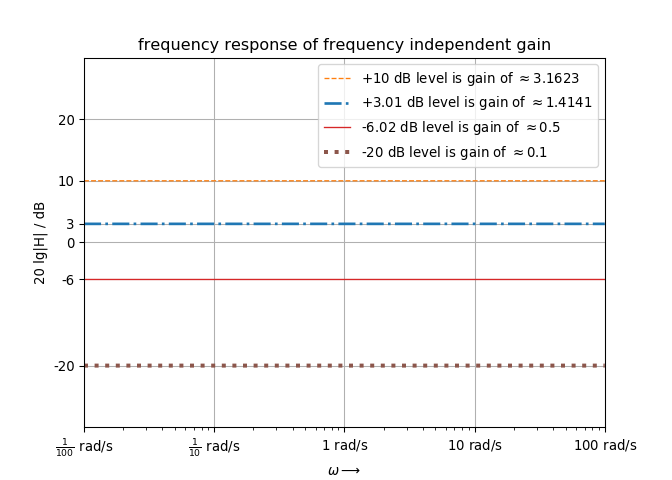
\includegraphics[width=0.5\textwidth]{../laplace_system_analysis/fig_bode_mag_gain}
}
\subfloat[Zeros and poles in origin of $s$-plane, \eq{eq:Hs_sorted_for_Bode_dB_origin}.\label{fig_bode_mag_origin_zeros_poles}]{%
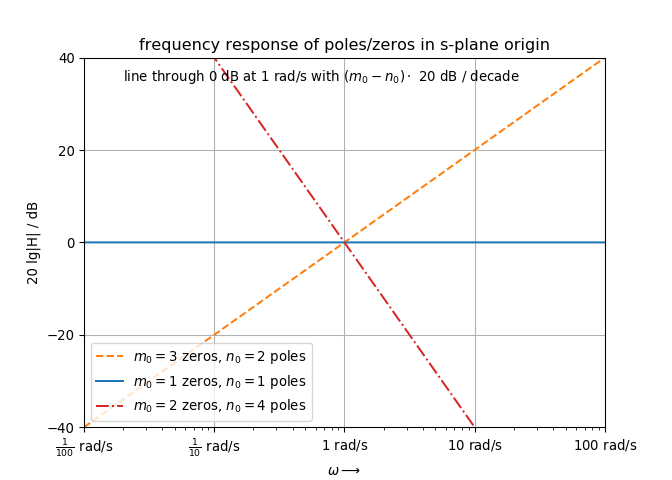
\includegraphics[width=0.5\textwidth]{../laplace_system_analysis/fig_bode_mag_origin_zeros_poles}
}

\subfloat[Single, real zero, \eq{eq:Hs_sorted_for_Bode_dB_zero}.\label{fig_bode_mag_single_zero}]{%
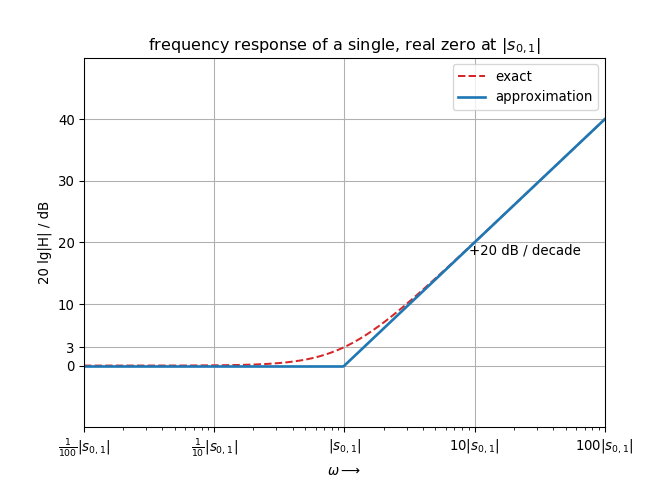
\includegraphics[width=0.5\textwidth]{../laplace_system_analysis/fig_bode_mag_single_zero}
}
\subfloat[Complex conjugate pair of zeros, \eq{eq:Hs_sorted_for_Bode_dB_cczero}.\label{fig_bode_mag_conj_zeros}]{%
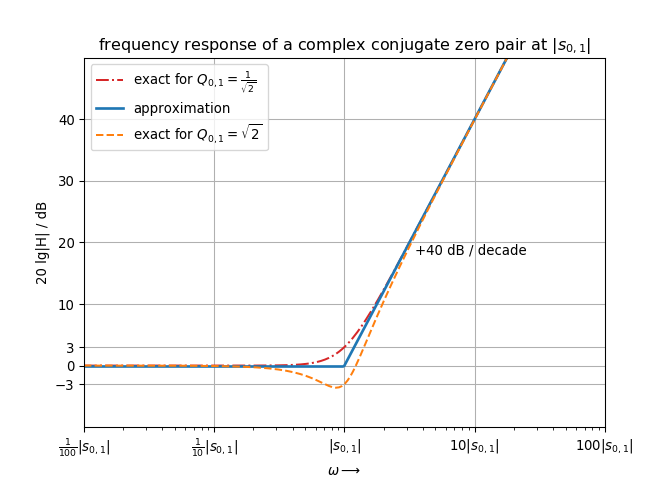
\includegraphics[width=0.5\textwidth]{../laplace_system_analysis/fig_bode_mag_conj_zeros}
}

\subfloat[Single, real pole, \eq{eq:Hs_sorted_for_Bode_dB_pole}.\label{fig_bode_mag_single_pole}]{%
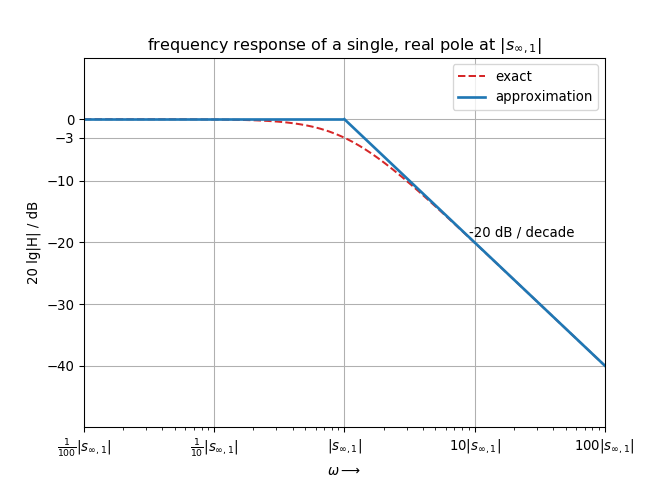
\includegraphics[width=0.5\textwidth]{../laplace_system_analysis/fig_bode_mag_single_pole}
}
\subfloat[Complex conjugate pair of poles, \eq{eq:Hs_sorted_for_Bode_dB_ccpole}.\label{fig_bode_mag_conj_poles}]{%
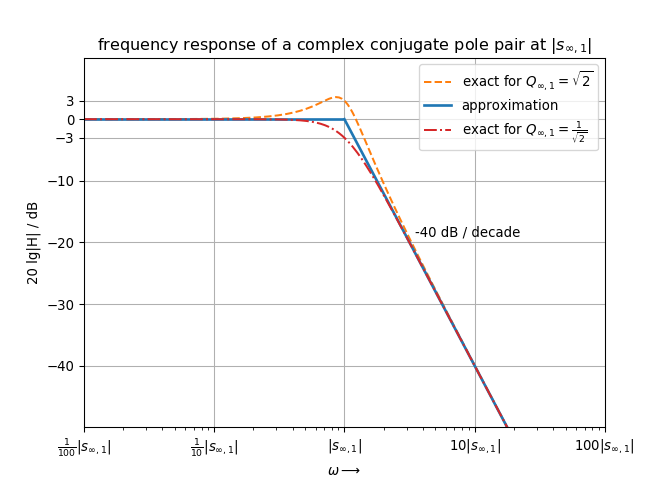
\includegraphics[width=0.5\textwidth]{../laplace_system_analysis/fig_bode_mag_conj_poles}
}
\caption{Magnitude frequency response of zero / pole prototypes for $s = \sigma + \im \omega$ with $\sigma=0$.
\texttt{bodeplot\_magnitude\_prototypes.ipynb}}
\label{fig:magbodeprototype}
\end{figure}

Recall that for the Laplace variable $s=\sigma + \im\omega$ a chosen  $\sigma=0$
leads to the Fourier transform of $H(s)$, i.e. only harmonic oscillating events
are considered, which we know as steady state.
This is precisely used to discuss the frequency response of an LTI system with
help of the Bode plot.
The level response of the Bode plot evaluates $20 \text{lg} |H(s)\big|_{s=\im \omega}|$.

The prototype systems \eq{eq:Hs_sorted_for_Bode_dB_gain} to
\eq{eq:Hs_sorted_for_Bode_dB_ccpole} exhibit an interesting characteristic,
when being plotted over a logarithmic frequency axis:
In the limiting cases, i.e. for frequencies much larger/smaller than around the pole/zero magnitude, the frequency response can be approximated by straight-line equations.
These approximations are visualised in Fig. \ref{fig:magbodeprototype}.
For example, for a single, real zero $s_{0,j}$ the prototype magnitude frequency response is $20 \text{lg}  \bigg|\frac{s}{s_{0,j}}-1\bigg|$
according to \eq{eq:Hs_sorted_for_Bode_dB_zero}.
For $|s| \ll |s_{0,j}|$, the value of one is dominating, yielding a line at 0 dB.
For $|s| \gg |s_{0,j}|$, the fraction is prevailing, yielding a line with a rise of 20 dB per decade (i.e. a tenfold increase of frequency).
The asymptotic characteristics changes exactly at $|s| = |s_{0,j}|$.
This is depicted in Fig. \ref{fig_bode_mag_single_zero}.



\clearpage
\subsubsection{Manual Logarithmic Diagram}
It is very helpful when we are able to draw a Bode plot sketch manually. In order
to do this we need to know how the logarithmic frequency axis is designed.
%
In SigSys either the $\log_{10}$ (w.r.t. frequency decade) or $\log_{2}$
(w.r.t. frequency octave) are commonly used.
%
Most important is to realized that each decade (10 times of a reference frequency)
or each octave (2 times of a reference frequency) takes always the same distance
on the x-axis.
%
This is the idea of the log plot.
%
Second, minor grid lines can be set up. For the $\log_10$ plot
this is standardized being the numbers from 1 to 10 within one decade.
\begin{center}
\begin{tikzpicture}
\centering
\def \tic {0.05}
\begin{scope}
\draw[->] (-0.5,0) -- (4.5,0) node[right]{$\log_{10} \frac{\omega}{\omega_r}$};
\draw[-] (0,-\tic) -- (0,+\tic) node[below]{$10^{-1}$};
\draw[-] (1,-\tic) -- (1,+\tic) node[below]{$10^{0}$};
\draw[-] (2,-\tic) -- (2,+\tic) node[below]{$10^{1}$};
\draw[-] (3,-\tic) -- (3,+\tic) node[below]{$10^{2}$};
\draw[-] (4,-\tic) -- (4,+\tic) node[below]{$10^{3}$};
\draw[->] (-0.5,0) -- (-0.5,2) node[above]{dB};
\draw[-] (-0.5-\tic,0.5) -- (-0.5+\tic,0.5) node[left]{20};
\draw[-] (-0.5-\tic,1.5) -- (-0.5+\tic,1.5) node[left]{40};
\draw[C0, -, ultra thick] (1,0.5) -- (2,1.5) node[right]{+20dB / decade};
\draw[-.,C7] (0.0,0.5) -- (0.0,1.5);
\draw[-.,C7] (0.30103,0.5) -- (0.30103,1.5);
\draw[-.,C7] (0.47712125,0.5) -- (0.47712125,1.5);
\draw[-.,C7] (0.60205999,0.5) -- (0.60205999,1.5);
\draw[-.,C7] (0.69897,0.5) -- (0.69897,1.5);
\draw[-.,C7] (0.77815125,0.5) -- (0.77815125,1.5);
\draw[-.,C7] (0.84509804,0.5) -- (0.84509804,1.5);
\draw[-.,C7] (0.90308999,0.5) -- (0.90308999,1.5);
\draw[-.,C7] (0.95424251,0.5) -- (0.95424251,1.5);
\draw[-.,C7] (1,0.5) -- (1,1.5);
\end{scope}
%
\begin{scope}[shift={(7,0)}]
\draw[->] (-0.5,0) -- (4.5,0) node[right]{$\log_{2}  \frac{\omega}{\omega_r}$};
\draw[-] (0,-\tic) -- (0,+\tic) node[below]{$2^{-1}$};
\draw[-] (1,-\tic) -- (1,+\tic) node[below]{$2^{0}$};
\draw[-] (2,-\tic) -- (2,+\tic) node[below]{$2^{1}$};
\draw[-] (3,-\tic) -- (3,+\tic) node[below]{$2^{2}$};
\draw[-] (4,-\tic) -- (4,+\tic) node[below]{$2^{3}$};
\draw[->] (-0.5,0) -- (-0.5,2) node[above]{dB};
\draw[-] (-0.5-\tic,0.5) -- (-0.5+\tic,0.5) node[left]{6};
\draw[-] (-0.5-\tic,1.5) -- (-0.5+\tic,1.5) node[left]{12};
\draw[C0, -, ultra thick] (1,0.5) -- (2,1.5) node[right]{$\approx$+6dB / octave};
\draw[-.,C7] (0.0,0.5) -- (0.0,1.5);
\draw[-.,C7] (0.13750352,0.5) -- (0.13750352,1.5);
\draw[-.,C7] (0.26303441,0.5) -- (0.26303441,1.5);
\draw[-.,C7] (0.37851162,0.5) -- (0.37851162,1.5);
\draw[-.,C7] (0.48542683,0.5) -- (0.48542683,1.5);
\draw[-.,C7] (0.5849625,0.5) -- (0.5849625,1.5);
\draw[-.,C7] (0.67807191,0.5) -- (0.67807191,1.5);
\draw[-.,C7] (0.76553475,0.5) -- (0.76553475,1.5);
\draw[-.,C7] (0.84799691,0.5) -- (0.84799691,1.5);
\draw[-.,C7] (0.92599942,0.5) -- (0.92599942,1.5);
\draw[-.,C7] (1,0.5) -- (1,1.5);
\end{scope}
\end{tikzpicture}
\end{center}

%log10 axis spacing:
%[0.         0.30103    0.47712125 0.60205999 0.69897    0.77815125
% 0.84509804 0.90308999 0.95424251 1.        ]
%log2 axis spacing:
%[0.         0.13750352 0.26303441 0.37851162 0.48542683 0.5849625
% 0.67807191 0.76553475 0.84799691 0.92599942 1.        ]


\begin{itemize}
  \item $\log_{10}$:
  (Standardised) grid lines for the first decade at
  \begin{align}
  10^{-1} \cdot [1,2,3,...,9,10]
  \end{align}
  to cover frequencies from $\omega=10^{-1} \omega_r$ to $\omega=10^1 \cdot 10^{-1} \omega_r= 10^0 \omega_r$
  can be drawn by the spacing values $\log_{10}[1,2,3,...,9,10]$
  along the relative line from 0 to 1 within this decade.
  \item $\log_{2}$:
  (Potentially meaningful) grid lines for the first octave at
  \begin{align}
  2^{-1} \cdot [1.0, 1.1, 1.2, 1.3,...,2.0]
  \end{align}
  to cover frequencies from $\omega=2^{-1} \omega_r$ to $\omega=2^1 \cdot 2^{-1} \omega_r = 2^0 \omega_r$
  can be drawn by the spacing values $\log_{2}[1,1.1,1.2,...,1.9,2]$
  along the relative line from 0 to 1 within this octave.
\end{itemize}
%
Often $\omega_r = 1$ is chosen.
In SigSys we often deal LTI systems that exhibit slopes of $\pm o \cdot 20$ dB / decade.
20 dB / decade correspond to $20\cdot \log_{10}(2) \approx 6.02$ dB / octave
in a $\log_2$ plot.
Then $\pm$40 dB / decade correspond to $\approx\pm$ 12 dB / octave and so on.





% %\bibliographystyle{IEEEtranSA.bst}
% %\bibliography{literature}
% \clearpage
% \bibliography{literatur}
% \end{document}
